%%%%%%%%%%%%%%%%%%%%%%%%%
% PACKAGES              %
%%%%%%%%%%%%%%%%%%%%%%%%%
\documentclass[]{report} % book|article|…

\usepackage[utf8x]{inputenc}    % accents
\usepackage{geometry}           % marges
\usepackage[francais]{babel}    % langue
\usepackage{graphicx}           % images
\usepackage{verbatim}           % texte préformaté
\usepackage{fancyhdr}           % fancy
\usepackage{filecontents}       % write file directly
\usepackage{csvsimple}          % csv reader
\usepackage{lastpage}	        % get number of last page
\usepackage{listings}           % source code 
\usepackage{url}                % clickable urls 
\usepackage{float}              % exact placing of figures
\usepackage{amsmath}            % fancy matrices
\usepackage{xkeyval}            % keywords arguments for newcommand
\usepackage{xifthen}            % provides \isempty test

% packages for graphics
\usepackage{fancybox}         
\usepackage{pgfplots}        
\usepackage{pgfplotstable}
\usepgfplotslibrary{dateplot}
\usepackage{pgfplots}

\definecolor{Gene0}{RGB}{250, 164, 1}
\definecolor{Gene1}{RGB}{128, 0, 128}
\definecolor{Gene2}{RGB}{255, 0, 0}
\definecolor{Gene3}{RGB}{58, 242, 75}
\definecolor{Gene4}{RGB}{8, 81, 156}
\definecolor{Diversity}{RGB}{0, 0, 0}

\pgfplotscreateplotcyclelist{list}{
        {Gene0},
        {Gene1},
        {Gene2},
        {Gene3},
        {Gene4},
        {Diversity}
}




%%%%%%%%%%%%%%%%%%%%%%%%%
% SIMULATION COMMAND    %
%%%%%%%%%%%%%%%%%%%%%%%%%
%This is needed for encapsulating.
%changes the catcode of @ so it
%can be used freely (not needed
%when writing a package)
\makeatletter

\define@cmdkey [SIMPAR] {fam} {generations} {}
\define@cmdkey [SIMPAR] {fam} {popsize}     {}
\define@cmdkey [SIMPAR] {fam} {parents}     {}
\define@cmdkey [SIMPAR] {fam} {seed}        {}
\define@cmdkey [SIMPAR] {fam} {mutationrate}{}
\define@cmdkey [SIMPAR] {fam} {initialpheno}{}
\define@cmdkey [SIMPAR] {fam} {link}        {}
 
\presetkeys [SIMPAR] {fam} {generations  = 200,
                            popsize      = 300,
                            parents      = 2,
                            seed         = 4223,
                            mutationrate = $10^{-4}$,
                            initialpheno = 11111,
                            link         = ?,
                           }{}

\newcommand{\simulationParameters}[1]{%
        \setkeys[SIMPAR]{fam}{#1}
        \begin{center}
                \begin{tabular}{|l|c||l|c|}
                \hline
                \textbf{Generations computed}   & \cmdSIMPAR@fam@generations    & \textbf{Population size}      & \cmdSIMPAR@fam@popsize        \\ \hline
                \textbf{Parent number}          & \cmdSIMPAR@fam@parents        & \textbf{Mutation rate}        & \cmdSIMPAR@fam@mutationrate   \\ \hline
                \textbf{Seed}                   & \cmdSIMPAR@fam@seed           & \textbf{Initial Phenotype}    & \cmdSIMPAR@fam@initialpheno   \\ \hline
                \textbf{Figure}                 & \ref{fig:\cmdSIMPAR@fam@link} & \textbf{Matrix}               & \ref{mat:\cmdSIMPAR@fam@link} \\ \hline
                \end{tabular}
        \end{center}
}

%Change again the @ catcode
%to normal
\makeatother




%%%%%%%%%%%%%%%%%%%%%%%%%
% PRÉAMBULE             %
%%%%%%%%%%%%%%%%%%%%%%%%%
%\title{Genomat\\PRJ Project Report}
%\author{Ostiane D'AUGUSTIN and Lucas BOURNEUF}
% laisser vide pour date de compilation
%\date{} 

% FORMAT PAGES         
\pagestyle{fancy} % nom du rendu (définit les lignes suivantes)
        \lhead{M1 BIG} % left head
        \chead{Genomat} % center head
        \rhead{2014/2015} % right head
        \lfoot{} % left foot
        \cfoot{\thepage/\pageref{LastPage}} % center foot
        \rfoot{} % right foot






%%%%%%%%%%%%%%%%%%%%%%%%%
% BEGIN                 %
%%%%%%%%%%%%%%%%%%%%%%%%%
\begin{document}
\begin{titlepage}
\newcommand{\HRule}{\rule{\linewidth}{0.5mm}}
\center
\textsc{\LARGE University of Rennes 1}\\[1.5cm]
\textsc{\large Master 1}\\[0.5cm] 
\textsc{\Large Bioinformatics and Genomics}\\[0.5cm] 

%----------------------------------------------------------------------------------------
%	TITLE SECTION
%----------------------------------------------------------------------------------------

\HRule \\[0.4cm]
{ \huge \bfseries Genomat}\\[0.4cm] % Title of your document
\HRule \\[1.5cm]
 
%----------------------------------------------------------------------------------------
%	AUTHOR SECTION
%----------------------------------------------------------------------------------------

\begin{minipage}{0.4\textwidth}
\begin{flushleft} \large
\emph{Authors:}\\
Lucas \textsc{Bourneuf}\\
Ostiane	\textsc{D'Augustin}
\end{flushleft}
\end{minipage}
~
\begin{minipage}{0.4\textwidth}
\begin{flushright} \large
\emph{Supervisors:} \\
Olivier \textsc{Dameron}
Yann \textsc{Le Cunff}\\
\end{flushright}
\end{minipage}\\[2cm]

%	DATE SECTION
{\large \today}\\[1cm] % Date, change the \today to a set date if you want to be precise

%	Link for Github
Source code available in \textsc{Public Domain} on github repository :\\ \url{https://github.com/Aluriak/Genomat}

%	LOGO SECTION
\vspace{1cm}

\includegraphics[width=0.6\textwidth]{rennes1_logo.png}\\[1cm] % Include a department/university logo - this will require the graphicx package

\end{titlepage}



%%%%%%%%%%%%%%%%%%%%%%%%%
% SECTION               %
%%%%%%%%%%%%%%%%%%%%%%%%%
\section*{Introduction}
	\paragraph*{}
	The aim of this project is to implement a genetic algorithm which will bring out the connexions between different genes, 
        their regulation networks, and some properties linked to, as well as their resistance to genes knock-out (KO).
	\paragraph*{}
        This project will study a famous genes network example, which has been highlighted by \textit{Wagner}. Wagner's genes network is an artificial genes network calculation model. 
        It has explained all the development and evolution process of genetic regulation networks. It has been first developed by Andreas Wagner in 1996, 
        and then used by several research teams in order to study genes network evolution, genes expression, etc.
	\paragraph*{}
        Main subject is an \textit{in silico} implementation of the Wagner's genes network, and observation of population's evolution over many generations, where an individual is a  genes network, also called \textit{genotype}. 
        Individuals will be submit to an evolutive process by the intermediary of their genes networks.




%%%%%%%%%%%%%%%%%%%%%%%%%
% SECTION               %
%%%%%%%%%%%%%%%%%%%%%%%%%
\section*{Project organization}
	\paragraph*{}
        The project follows a Python-like packaging, with the main program launchable as a package. (\textit{python -m genomat})
        Many parameters can be sended through command-line arguments, or configuration file. Some of them are used for comparison and to study Wagner's model.
        \textit{python -m genomat --help} show all applicable options.\\
        Outputs are mainly in \textsc{csv format} (notabily those provided for statistics).

	\paragraph*{}
        A second and incomplete implementation of Genomat is available under the name of \textit{genomat\_func}. 
        This implementation is only here as a proof of concept that use a functionnal approach.

	\paragraph*{}
        Used technologies :
        \begin{itemize}
                \item \textbf{python} as the main language (version 3.4);
                \item \textbf{docopt} as command-line arguments parser;
                \item \textbf{doctest} for unit tests in some docstrings (see \textsc{unittests.py} file);
                \item \textbf{numpy} for manage matrix (and notabily multiplications) until Python 3.5 interpreter is available;
                \item \textbf{latex} for present report, with pgfplot module for automatic data vizualization generation;
                \item \textbf{pylint} for source code profiling and UML generation;
                \item \textbf{make} for automatize simulations, tests, etc;
        \end{itemize}





%%%%%%%%%%%%%%%%%%%%%%%%%
% SECTION               %
%%%%%%%%%%%%%%%%%%%%%%%%%
\section*{Source code architecture}
	\paragraph*{}
        Genomat is cut in modules as shown in Figure~\ref{fig:umldiag}, and described below.
        \begin{itemize}
                \item \textbf{main} implements a simple and efficient interface that allow command-line arguments;
                \item \textbf{config} management of configurations : files, options, flags, serialization;
                \item \textbf{gene network} definition of an individual, encapsulation of numpy matrix system;
                \item \textbf{population} a list of individuals that provides many data access and call stats modules as an observer;
                \item \textbf{stats} observer of population that tests it and generates, if asked, data in targeted files;
                \item \textbf{progress bar} dumb and simple implementation of a progress bar, designed to be replaced later;
        \end{itemize}

        \begin{figure}[H] 
                \centering
                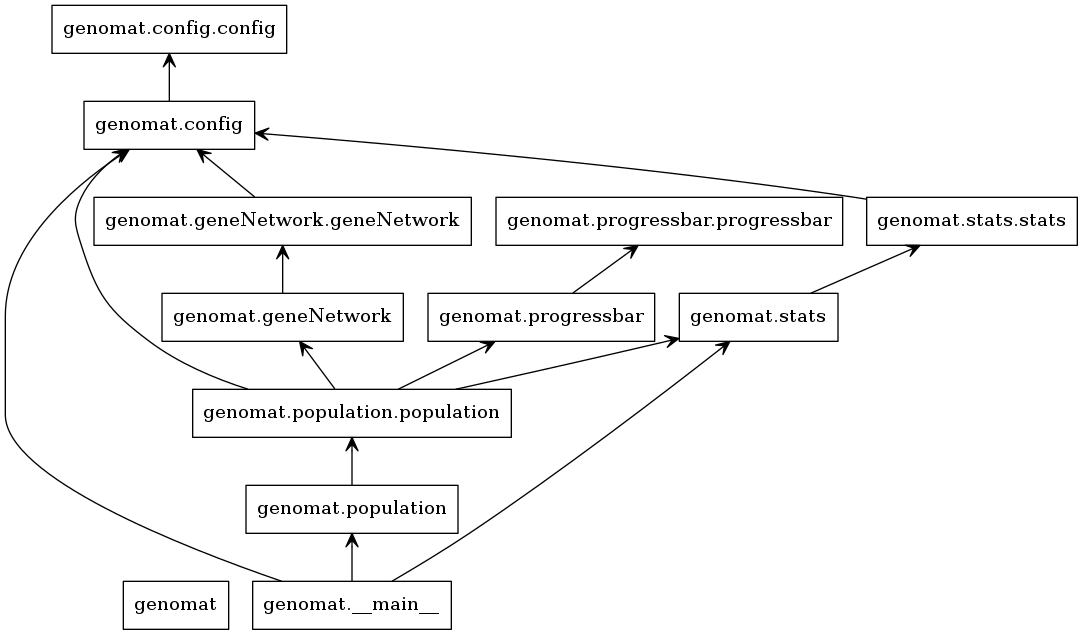
\includegraphics[width=\textwidth]{packages_genomat.png}
                \caption{\footnotesize Modules of Genomat architecture, without externals ones (numpy, docopt).}
                \label{fig:umldiag}
        \end{figure}

	\paragraph*{}
        Architecture is designed with the help of some patterns. 
        Notabily, Observer Pattern provides a total and powerful flexibility about what is watched in simulations.
        An easy solution for extends statistics study and do interesting things like phylogenetic trees is create an Observer dedicated to that task.
        The current observers are basics, but necessary for a first approach.

        \paragraph*{}
        The Genomat source code is placed in the public domain. Feel free to use it for improve implementations, add observers and crunsh your own data ! 



%%%%%%%%%%%%%%%%%%%%%%%%%
% SECTION               %
%%%%%%%%%%%%%%%%%%%%%%%%%
\section{Watchables}
    \paragraph*{}
    Main data generated results of gene KO, for each gene at each generation. 
    A diversity ratio is also computed at each generation.
    \paragraph*{}
     First, as there was no mutation rate given, exploited simulations use a mutation rate from $10^{-0}$ to $10^{-10}$, 
     with a constant population size of 300 individuals and 200 generations.\\
     For each gene, the survavibility ratio is computed. \\
     The survivability ratio is defined as $S_g = \frac{KO_g}{population_{size}}$ 
     with $KO_g$ as the number of individuals still viable after the KO of gene g.



%%%%%%%%%%%%%%%%%%%%%%%%%
% SECTION               %
%%%%%%%%%%%%%%%%%%%%%%%%%
\newpage
\section*{Results through graphics}
%%%%%%%%%%%%%%%%%%%%%%%%%%%%%%%%%%%%%%%%%%%%%%%%%%%%%%%%%%%%%%%%%%%%%%%%%%%%%%%%%%%%%%%%%%%%%%
% SUBSECTION 
%%%%%%%%%%%%%%%%%%%%%%%%%%%%%%%%%%%%%%%%%%%%%%%%%%%%%%%%%%%%%%%%%%%%%%%%%%%%%%%%%%%%%%%%%%%%%%
\newpage
\subsection{Telltale}
    \paragraph*{}
    The used telltale follows the next rules :\\
    \simulationParameters{link=telltale}
    \begin{figure}[H] 
      \centering
      \begin{tikzpicture}
          \begin{axis}[
                  %,no mark % retract marks at point location
                  ,xlabel={Generations}
                  ,ylabel={Survivability ratio}
                  ,grid=major % grid on all axis
                  ,axis lines=left
                  ,ymajorgrids
                  ,legend style={legend pos=south west}
                  ,cycle list name=list
              ]
              \addplot table [col sep=comma,x=generationnumber,y=viabilityratio0] {ps300xg200xmr1-10-4.csv};
              \addplot table [col sep=comma,x=generationnumber,y=viabilityratio1] {ps300xg200xmr1-10-4.csv};
              \addplot table [col sep=comma,x=generationnumber,y=viabilityratio2] {ps300xg200xmr1-10-4.csv};
              \addplot table [col sep=comma,x=generationnumber,y=viabilityratio3] {ps300xg200xmr1-10-4.csv};
              \addplot table [col sep=comma,x=generationnumber,y=viabilityratio4] {ps300xg200xmr1-10-4.csv};
              \addplot[line width=1.0pt, mark=x] 
                       table [col sep=comma,x=generationnumber,y=diversity]       {ps300xg200xmr1-10-4.csv};
              \legend{Gene 0, Gene 1, Gene 2, Gene 3, Gene 4, Diversity}
          \end{axis}
      \end{tikzpicture}
      \caption{\footnotesize Resistance to gene KO survivability ratio, over 200 generations, with a population of 300 individuals and a mutation rate of $10^{-4}$, use as telltale}
      \label{fig:telltale}
    \end{figure}
    \paragraph*{}
    The mutation rate of $10^{-4}$ is used as the default parameter because its a medium value, which can be a "natural" mutation rate, to which it will be easy to compare the other data.
    \paragraph*{}
    First, genes seems to have rather the same conduct : their resistance to KO survivability ratio first increase and then stabilize about more or less 1. 
    But there are two different conducts in that global trend. In one hand, genes 1, 3, 4 and even later gene 2 reach a resistance to KO survivability ratio equals to 1. 
    It means that those genes, even once KO, do not avoid the individual's survival. In the other hand, the gene 0 never reaches resistance to KO survivability ratio of 1. 
    It approaches the 150th and the 160th generations, but does not reaches it for all that. It means that this gene 0 is more essential for the individual's survival.
    \paragraph*{}
    As a result, the diversity is slowly decreasing during the 50 first generations. 
    Then, it decreases rather fastly from 1 to 0.4 up to the 150th generation, where it finaly stabilizes around 0.35. 
    Indeed, as there is only one gene to be essential, and as the mutation rate is pretty low, the global population phenotype is stabilizing, which lowers the diversity.

    \begin{figure}[H] 
            \centering
            \small
    $
            \begin{pmatrix}
                150 +- 190 & -2 +- 335 & 177 +- 295 & 23 +- 175 & 4 +- 1426 \\
                146 +- 10206 & 76 +- 9686 & -18 +- 4078 & 52 +- 9762 & -40 +- 2479 \\
                -4 +- 0 & -33 +- 401 & 208 +- 608 & -9 +- 85 & 42 +- 1103 \\
                -67 +- 4290 & -17 +- 472 & -56 +- 186 & 57 +- 1245 & 67 +- 3686 \\
                -7 +- 6196 & -53 +- 13893 & 33 +- 1259 & 2 +- 692 & 91 +- 1449 9 
            \end{pmatrix}
    $
            \caption{\footnotesize Matrix generated with the data of the telltale last generation.}
            \label{mat:telltale}
    \end{figure}
    \paragraph*{}
    A big value indicates a big gene influence on the other, and a small value, a small influence. If it is a positive value, the gene is a promoter, and, if it is a negative value, its a down-regulator.
    A $m +- v$ notation show that the gene affect the other, in all the population, with an average value of m and a variance of v.
    First consequence of that observation : variance of 0 shows an identical gene regulation value in all the population.
    \paragraph*{}
    All the positions are not interesting, but some can be easily commented :
    \begin{itemize}
            \item The last data of the first line (4 +- 1428) seems that the gene 4 have both a role of promotor and regulator for the gene 4 (average near to 0, high variance).
        \item The first data of the third line (-4 +- 0) means that the gene 2 performs a small down-regulation on the gene 2 (influence = -4), and, because of the variability of 0, its a universal behavior.
    \end{itemize}
    \paragraph*{}
    In all simulations, many genes will present an important variation of genes regulation, but some of them will be conserved by all genes networks.
    

    
    
%%%%%%%%%%%%%%%%%%%%%%%%%%%%%%%%%%%%%%%%%%%%%%%%%%%%%%%%%%%%%%%%%%%%%%%%%%%%%%%%%%%%%%%%%%%%%%
% SUBSECTION 
%%%%%%%%%%%%%%%%%%%%%%%%%%%%%%%%%%%%%%%%%%%%%%%%%%%%%%%%%%%%%%%%%%%%%%%%%%%%%%%%%%%%%%%%%%%%%%
\newpage
\subsection{Telltale with another seed}
    \paragraph*{}
    Just for verify that choice of seed is not critical for results, a run of the telltale with a different seed is performed : \\
    \simulationParameters{link=telltaleAlt, seed=587603}
    \begin{figure}[H] 
      \centering
      \begin{tikzpicture}
          \begin{axis}[
                  %,no mark % retract marks at point location
                  ,xlabel={Generations}
                  ,ylabel={Survivability ratio}
                  ,grid=major % grid on all axis
                  ,axis lines=left
                  ,ymajorgrids
                  ,legend style={legend pos=south west}
                  ,cycle list name=list
              ]
              \addplot table [col sep=comma,x=generationnumber,y=viabilityratio0] {ps300xg200xmr1-10-4xsd587603.csv};
              \addplot table [col sep=comma,x=generationnumber,y=viabilityratio1] {ps300xg200xmr1-10-4xsd587603.csv};
              \addplot table [col sep=comma,x=generationnumber,y=viabilityratio2] {ps300xg200xmr1-10-4xsd587603.csv};
              \addplot table [col sep=comma,x=generationnumber,y=viabilityratio3] {ps300xg200xmr1-10-4xsd587603.csv};
              \addplot table [col sep=comma,x=generationnumber,y=viabilityratio4] {ps300xg200xmr1-10-4xsd587603.csv};
              \addplot[line width=1.0pt, mark=x] 
                       table [col sep=comma,x=generationnumber,y=diversity]       {ps300xg200xmr1-10-4xsd587603.csv};
              \legend{Gene 0, Gene 1, Gene 2, Gene 3, Gene 4, Diversity}
          \end{axis}
      \end{tikzpicture}
      \caption{\footnotesize Resistance to gene KO survivability ratio, over 200 generations, with a population of 300 individuals and a mutation rate of $10^{-4}$, use as telltale}
      \label{fig:telltaleAlt}
    \end{figure}
    This matrix is generated with of the last generation, and shows the medium influence of each genes on the others over the whole population and the variability around the pass mark. 
    \paragraph*{}
    As expected, two simulations that differs only by pseudo-random number generation will generate close results. 
    In fact, even with many runs of a simulation with a random seed, results always converge to a single solution, with some variations.
    (important gene and time before stabilization)

    \begin{figure}[H] 
            \centering
            \small
    $
            \begin{pmatrix}
                104 +- 0 & -14 +- 0 & 82 +- 0 & -29 +- 30 & 21 +- 0 \\
                1 +- 725 & 145 +- 1674 & 15 +- 201 & -4 +- 16 & -57 +- 613 \\
                -81 +- 3247 & 134 +- 12750 & 42 +- 2187 & 50 +- 27995 & -28 +- 2354 \\
                7 +- 2038 & -98 +- 5920 & 139 +- 1765 & 229 +- 1634 & -105 +- 4875 \\
                -28 +- 4677 & 93 +- 1528 & -39 +- 3049 & -31 +- 1197 & 229 +- 1967 
            \end{pmatrix}
    $
            \caption{\footnotesize Matrix generated with the data of the last generation. First gene is almost totally conserved in all individuals of the population.}
            \label{mat:telltaleAlt}
    \end{figure}
    \paragraph*{}
    Interesting case : the first gene is almost totally conserved by all individuals. Others genes have very variable regulations values.
    Last genes show average values near from 0.
    


%%%%%%%%%%%%%%%%%%%%%%%%%%%%%%%%%%%%%%%%%%%%%%%%%%%%%%%%%%%%%%%%%%%%%%%%%%%%%%%%%%%%%%%%%%%%%%
% SUBSECTION 
%%%%%%%%%%%%%%%%%%%%%%%%%%%%%%%%%%%%%%%%%%%%%%%%%%%%%%%%%%%%%%%%%%%%%%%%%%%%%%%%%%%%%%%%%%%%%%
    \newpage
\subsection{Mutation rate variation}
    \paragraph*{}
    Parameters for the first experience :\\
    \simulationParameters{mutationrate=$10^{-0}$, link=ps300xg200xmr1-10-0}
    \begin{figure}[H] 
      \centering
      \begin{tikzpicture}
          \begin{axis}[
                  %,no mark % retract marks at point location
                  ,xlabel={Generations}
                  ,ylabel={Survivability ratio}
                  ,grid=major % grid on all axis
                  ,axis lines=left
                  ,ymajorgrids
                  ,legend style={legend pos=south east}
                  ,cycle list name=list
              ]
              \addplot table [col sep=comma,x=generationnumber,y=viabilityratio0] {ps300xg200xmr1-10-0.csv};
              \addplot table [col sep=comma,x=generationnumber,y=viabilityratio1] {ps300xg200xmr1-10-0.csv};
              \addplot table [col sep=comma,x=generationnumber,y=viabilityratio2] {ps300xg200xmr1-10-0.csv};
              \addplot table [col sep=comma,x=generationnumber,y=viabilityratio3] {ps300xg200xmr1-10-0.csv};
              \addplot table [col sep=comma,x=generationnumber,y=viabilityratio4] {ps300xg200xmr1-10-0.csv};
              \addplot[line width=1.0pt, mark=x] 
                       table [col sep=comma,x=generationnumber,y=diversity]       {ps300xg200xmr1-10-0.csv};
              \legend{Gene 0, Gene 1, Gene 2, Gene 3, Gene 4, Diversity}
          \end{axis}
      \end{tikzpicture}
      \caption{\footnotesize Resistance to gene KO survivability ratio, over 200 generations, with a population of 300 individuals and a mutation rate of 1}
      \label{fig:ps300xg200xmr1-10-0}
    \end{figure}
    \paragraph*{}
    A mutation rate of 1 means that each gene of each individual of each generation will mutate. Its a limit case that show a constantly different population.
    \paragraph*{}
    As each gene mutates, there is no constant resistance to gene KO survivability ratio stabilization, as we could see for the telltale. 
    Each gene is more or less essential. The Resistance to gene KO never stabilize to 1, 
    however, all the lines are beyond 0.9, and never decrease to a lower value. 
    As each gene mutates, the diversity is very high (constantly equals to 1).

    \begin{figure}[H] 
            \centering
            \small
    $
            \begin{pmatrix}
                304 +- 8526 & -39 +- 33750 & 119 +- 15040 & 15 +- 8066 & -26 +- 4692 \\
                138 +- 21689 & 291 +- 7052 & 94 +- 33661 & 55 +- 10078 & 62 +- 17995 \\
                326 +- 9222 & 121 +- 2688 & 156 +- 10334 & -90 +- 9970 & -234 +- 19612 \\
                87 +- 6326 & -78 +- 9487 & 63 +- 5292 & 223 +- 6283 & 128 +- 14690 \\
                15 +- 25929 & 58 +- 25518 & 2 +- 10437 & -80 +- 5527 & 241 +- 9406 
            \end{pmatrix}
    $
            \caption{\footnotesize Matrix generated with the data of the last generation}
            \label{mat:ps300xg200xmr1-10-0}
    \end{figure}
    \paragraph*{}
    Averaged regulation values stay near 0 (2 to 326 in absolute values), but variances are very high. There is probably a direct correlation to the diversity which is still 1 at the end of the 200 generations. 
    In other words, each genotype is different, and no genes have a universal influence on another (promotor or regulator).\\
    It shows the range of possibilities for assure genomes viability.
    
    
    \newpage
    \paragraph*{}
    Parameters for the next experience :\\
    \simulationParameters{mutationrate=$10^{-1}$, link=ps300xg200xmr1-10-1}
    \begin{figure}[H] 
    \centering
    \begin{tikzpicture}
       \begin{axis}[
                  %,no mark % retract marks at point location
                  ,xlabel={Generations}
                  ,ylabel={Survivability ratio}
                  ,grid=major % grid on all axis
                  ,axis lines=left
                  ,ymajorgrids
                  ,legend style={legend pos=south east}
                  ,cycle list name=list
              ]
              \addplot table [col sep=comma,x=generationnumber,y=viabilityratio0] {ps300xg200xmr1-10-1.csv};
              \addplot table [col sep=comma,x=generationnumber,y=viabilityratio1] {ps300xg200xmr1-10-1.csv};
              \addplot table [col sep=comma,x=generationnumber,y=viabilityratio2] {ps300xg200xmr1-10-1.csv};
              \addplot table [col sep=comma,x=generationnumber,y=viabilityratio3] {ps300xg200xmr1-10-1.csv};
              \addplot table [col sep=comma,x=generationnumber,y=viabilityratio4] {ps300xg200xmr1-10-1.csv};
              \addplot[line width=1.0pt, mark=x] 
                       table [col sep=comma,x=generationnumber,y=diversity]       {ps300xg200xmr1-10-1.csv};
              \legend{Gene 0, Gene 1, Gene 2, Gene 3, Gene 4, Diversity}
          \end{axis}
      \end{tikzpicture}
      \caption{\footnotesize Resistance to gene KO survivability ratio, over 200 generations, with a population of 300 individuals and a mutation rate of $10^{-1}$}
      \label{fig:ps300xg200xmr1-10-1}
    \end{figure}
    \paragraph*{}
    A mutation rate of $10^{-1}$ is still very high for a natural population, and the global conduct is similar to the previous graph one's. 
    However, the resistance to gene KO survivability ratios are lower than the previous. 
    As the mutation rate is lower, there is a bit more phenotype stabilization, and thus, a gene can easier become essential. 
    For example, it is the case of the gene 0, which waits for the 60th generation to become unessential and stabilize around 1; 
    contrary to gene 1 which is first unessential, and becomes more and more essential as the time spends.
    \paragraph*{}
    Nevertheless, the diversity is still very high (constant equals to 1), which explains the pretty good resistance to gene KO survivability ratios.
   

    \begin{figure}[H] 
            \centering
            \small
    $
            \begin{pmatrix}
                98 +- 6039 & -26 +- 2711 & 28 +- 3244 & 75 +- 2903 & 13 +- 926 \\
                -39 +- 2815 & 152 +- 3468 & 45 +- 700 & -33 +- 796 & -45 +- 658 \\
                -31 +- 2053 & 71 +- 9285 & 120 +- 6335 & 9 +- 5160 & 80 +- 6374 \\
                -22 +- 4187 & -53 +- 612 & 27 +- 693 & 68 +- 785 & 152 +- 2428 \\
                39 +- 3960 & 47 +- 4600 & 14 +- 5258 & 2 +- 1785 & 116 +- 1672 
            \end{pmatrix}
    $
            \caption{\footnotesize Matrix generated with the data of the last generation}
            \label{mat:ps300xg200xmr1-10-1}
    \end{figure}
    \paragraph*{}
    The averaged influences variation is smaller than the previous case (2 to 152 in absolute values) from a gene to an other, but the variability around those values are still very high. 
    We can correlate this fact to the diversity which is still 1 at the end of the 200 generations. 
    There are a lot of different genotypes (genes networks) and then a lot of different phenotypes, with different genes influence from an individual to another.
    
    
    \newpage
    \paragraph*{}
    Parameters for the next experience :\\
    \simulationParameters{mutationrate=$10^{-2}$, link=ps300xg200xmr1-10-2}
    \begin{figure}[H] 
    \centering
    \begin{tikzpicture}
        \begin{axis}[
                  %,no mark % retract marks at point location
                  ,xlabel={Generations}
                  ,ylabel={Survivability ratio}
                  ,grid=major % grid on all axis
                  ,axis lines=left
                  ,ymajorgrids
                  ,legend style={legend pos=south east}
                  ,cycle list name=list
              ]
              \addplot table [col sep=comma,x=generationnumber,y=viabilityratio0] {ps300xg200xmr1-10-2.csv};
              \addplot table [col sep=comma,x=generationnumber,y=viabilityratio1] {ps300xg200xmr1-10-2.csv};
              \addplot table [col sep=comma,x=generationnumber,y=viabilityratio2] {ps300xg200xmr1-10-2.csv};
              \addplot table [col sep=comma,x=generationnumber,y=viabilityratio3] {ps300xg200xmr1-10-2.csv};
              \addplot table [col sep=comma,x=generationnumber,y=viabilityratio4] {ps300xg200xmr1-10-2.csv};
              \addplot[line width=1.0pt, mark=x] 
                       table [col sep=comma,x=generationnumber,y=diversity]       {ps300xg200xmr1-10-2.csv};
              \legend{Gene 0, Gene 1, Gene 2, Gene 3, Gene 4, Diversity}
          \end{axis}
      \end{tikzpicture}
      \caption{\footnotesize Resistance to gene KO survivability ratio, over 200 generations, with a population of 300 individuals and a mutation rate of $10^{-2}$}
      \label{fig:ps300xg200xmr1-10-2}
    \end{figure}
    \paragraph*{}
    A mutation rate of $10^{-2}$ is still a pretty high mutation rate, and the conduct is very similar to the previous graph one's. 
    However, a few variation in the diversity appears, due to the fact that there small stabilizations on the global phenotype.

    \begin{figure}[H] 
            \centering
            \small
    $
            \begin{pmatrix}
                201 +- 5007 & -10 +- 3188 & 35 +- 8854 & -10 +- 7485 & 51 +- 666 \\
                55 +- 106 & 298 +- 215 & 61 +- 227 & 35 +- 100 & 80 +- 265 \\
                41 +- 743 & 119 +- 1950 & 109 +- 3238 & -132 +- 7931 & 54 +- 1729 \\
                -62 +- 567 & -39 +- 1281 & -16 +- 93 & 167 +- 4186 & -55 +- 613 \\
                -164 +- 10949 & -82 +- 2716 & 106 +- 1495 & -84 +- 12073 & 162 +- 5029  
            \end{pmatrix}
    $
            \caption{\footnotesize Matrix generated with the data of the last generation}
            \label{mat:ps300xg200xmr1-10-2}
    \end{figure}    
    \paragraph*{}
    The averaged influence vary a bit more than the previous experience (10 to 298 in absolute values) from a gene to an other, but the variability around those values are still very high. 
    There is a possible correlation this fact to the diversity which is almost 1 at the end of the 200 generations. 
    There are a lot of different genotypes (genes networks) and then a lot of different phenotypes, with different genes influence from an individual to another.

      
    \newpage
    \paragraph*{}
    Parameters for the next experience :\\
    \simulationParameters{mutationrate=$10^{-5}$, link=ps300xg200xmr1-10-5}
    \begin{figure}[H] 
    \centering
    \begin{tikzpicture}
        \begin{axis}[
                  %,no mark % retract marks at point location
                  ,xlabel={Generations}
                  ,ylabel={Survivability ratio}
                  ,grid=major % grid on all axis
                  ,axis lines=left
                  ,ymajorgrids
                  ,legend style={legend pos=south west}
                  ,cycle list name=list
              ]
              \addplot table [col sep=comma,x=generationnumber,y=viabilityratio0] {ps300xg200xmr1-10-5.csv};
              \addplot table [col sep=comma,x=generationnumber,y=viabilityratio1] {ps300xg200xmr1-10-5.csv};
              \addplot table [col sep=comma,x=generationnumber,y=viabilityratio2] {ps300xg200xmr1-10-5.csv};
              \addplot table [col sep=comma,x=generationnumber,y=viabilityratio3] {ps300xg200xmr1-10-5.csv};
              \addplot table [col sep=comma,x=generationnumber,y=viabilityratio4] {ps300xg200xmr1-10-5.csv};
              \addplot[line width=1.0pt, mark=x] 
                       table [col sep=comma,x=generationnumber,y=diversity]       {ps300xg200xmr1-10-5.csv};
              \legend{Gene 0, Gene 1, Gene 2, Gene 3, Gene 4, Diversity}
          \end{axis}
      \end{tikzpicture}
      \caption{\footnotesize Resistance to gene KO survivability ratio, over 200 generations, with a population of 300 individuals and a mutation rate of $10^{-5}$}
      \label{fig:ps300xg200xmr1-10-5}
    \end{figure}
    \paragraph*{}
    A mutation rate of $10^{-5}$ is a usual mutation rate in a natural population. This result is thus very insteresting because it really reflects the global conducts of a natural population 
    (as far as we can consider as natural a population composed of only five genes).
    \paragraph*{}
    With this mutation rate, the five genes have a very similar conduct. Their resistance to KO increase over the 50 first generation, and then, due to the weak mutation rate, stabilized at 1 without decreasing.
    \paragraph*{} 
    As a result of the genes conduct, the diversity first decreases very slowly during the 50 first generations, and then fall fastly to 0.35. 

    \begin{figure}[H] 
            \centering
            \small
    $
            \begin{pmatrix}
                  193 +- 211    & 43 +- 1393    & 24 +- 80      & -80 +- 570    & 7 +- 362 \\
                  92 +- 1732    & 155 +- 75     & 106 +- 7319   & 105 +- 8293   & -15 +- 1104 \\
                  24 +- 3515    & 17 +- 3064    & 107 +- 9182   & 14 +- 1100    & -17 +- 1364 \\
                  -100 +- 1215  & 185 +- 7793   & 84 +- 415     & 164 +- 582    & -91 +- 191 \\
                  29 +- 2611    & 92 +- 1664    & 2 +- 2128     & 39 +- 5680    & 151 +- 499 
            \end{pmatrix}
    $
            \caption{\footnotesize Matrix generated with the data of the last generation}
            \label{mat:ps300xg200xmr1-10-5}
    \end{figure}
    \paragraph*{}
    All average genes values are near 0, with an high variance that allow all gene to promotes or regulates others. 
    The first gene show a little less variable regulation value.


    \paragraph*{}
    Parameters for the next experience :\\
    \simulationParameters{mutationrate=$10^{-10}$, link=ps300xg200xmr1-10-10}
    \begin{figure}[H] 
    \centering
    \begin{tikzpicture}
        \begin{axis}[
                  %,no mark % retract marks at point location
                  ,xlabel={Generations}
                  ,ylabel={Survivability ratio}
                  ,grid=major % grid on all axis
                  ,axis lines=left
                  ,ymajorgrids
                  ,legend style={legend pos=south west}
                  ,cycle list name=list
              ]
              \addplot table [col sep=comma,x=generationnumber,y=viabilityratio0] {ps300xg200xmr1-10-10.csv};
              \addplot table [col sep=comma,x=generationnumber,y=viabilityratio1] {ps300xg200xmr1-10-10.csv};
              \addplot table [col sep=comma,x=generationnumber,y=viabilityratio2] {ps300xg200xmr1-10-10.csv};
              \addplot table [col sep=comma,x=generationnumber,y=viabilityratio3] {ps300xg200xmr1-10-10.csv};
              \addplot table [col sep=comma,x=generationnumber,y=viabilityratio4] {ps300xg200xmr1-10-10.csv};
              \addplot[line width=1.0pt, mark=x] 
                       table [col sep=comma,x=generationnumber,y=diversity]       {ps300xg200xmr1-10-10.csv};
              \legend{Gene 0, Gene 1, Gene 2, Gene 3, Gene 4, Diversity}
          \end{axis}
      \end{tikzpicture}
      \caption{\footnotesize Resistance to gene KO survivability ratio, over 200 generations, with a population of 300 individuals and a mutation rate of $10^{-10}$}
      \label{fig:ps300xg200xmr1-10-10}
    \end{figure}
    \paragraph*{}
    A mutation rate of $10^{-10}$ lead to the same profile as the previous graph, for the experimentation with a mutation rate of $10^{-5}$. Those results suppose that 
    for a given population size and a given genes network, we will always obtain the same results using mutation rates low enough.
    \paragraph*{}
    A low mutation rate provides a very stable population for mutation propagation. 
    A beneficial mutation will have more time for be propagated in the population than in the previous simulations. Moreover, it will be mainly propagated "as is", 
    without other mutations. In a context of higher mutation rate, a mutation, before be propagated to all population, will be modified or complemented by another mutation.

    \begin{figure}[H] 
            \centering
            \small
    $
          \begin{pmatrix}
                183 +- 1857 & 18 +- 629 & 4 +- 2699 & -67 +- 3022 & 28 +- 1536 \\
                50 +- 0 & 163 +- 0 & -82 +- 0 & 3 +- 0 & 7 +- 0 \\
                62 +- 1789 & 53 +- 513 & 64 +- 3193 & 45 +- 1050 & 7 +- 154 \\
                -71 +- 5017 & 52 +- 852 & 52 +- 66 & 96 +- 3062 & 37 +- 8393 \\
                -8 +- 1308 & -1 +- 2278 & 48 +- 456 & -71 +- 573 & 162 +- 101 
          \end{pmatrix}
    $
            \caption{\footnotesize Matrix generated with the data of the last generation}
            \label{mat:ps300xg200xmr1-10-10}
    \end{figure}
    \paragraph*{}
    The gene 1 as a very conserved influence on other genes, with a variability of 0. That means that there is only one possible genotype for this gene and its interactions with the other genes.
    
    
%%%%%%%%%%%%%%%%%%%%%%%%%%%%%%%%%%%%%%%%%%%%%%%%%%%%%%%%%%%%%%%%%%%%%%%%%%%%%%%%%%%%%%%%%%%%%%
% SUBSECTION 
%%%%%%%%%%%%%%%%%%%%%%%%%%%%%%%%%%%%%%%%%%%%%%%%%%%%%%%%%%%%%%%%%%%%%%%%%%%%%%%%%%%%%%%%%%%%%%
    \newpage
\subsection{Parents number variation}
    \paragraph*{}
    Parameters for the next experience :\\
    \simulationParameters{parents=300, link=ps300xg200xmr1-10-4xprt300}
    \begin{figure}[H] 
    \centering
        \begin{tikzpicture}
            \begin{axis}[
                  %,no mark % retract marks at point location
                  ,xlabel={Generations}
                  ,ylabel={Survivability ratio}
                  ,grid=major % grid on all axis
                  ,axis lines=left
                  ,ymajorgrids
                  ,legend style={legend pos=south west}
                  ,cycle list name=list
              ]
              \addplot table [col sep=comma,x=generationnumber,y=viabilityratio0] {ps300xg200xmr1-10-4xprt300.csv};
              \addplot table [col sep=comma,x=generationnumber,y=viabilityratio1] {ps300xg200xmr1-10-4xprt300.csv};
              \addplot table [col sep=comma,x=generationnumber,y=viabilityratio2] {ps300xg200xmr1-10-4xprt300.csv};
              \addplot table [col sep=comma,x=generationnumber,y=viabilityratio3] {ps300xg200xmr1-10-4xprt300.csv};
              \addplot table [col sep=comma,x=generationnumber,y=viabilityratio4] {ps300xg200xmr1-10-4xprt300.csv};
              \addplot[line width=1.0pt, mark=x] 
                       table [col sep=comma,x=generationnumber,y=diversity]       {ps300xg200xmr1-10-4xprt300.csv};
              \legend{Gene 0, Gene 1, Gene 2, Gene 3, Gene 4, Diversity}
          \end{axis}
      \end{tikzpicture}
      \caption{\footnotesize Resistance to gene KO survivability ratio, over 200 generations, with a population of 300 individuals, a mutation rate of $10^{-4}$, and a parents number equals to the population size}
      \label{fig:ps300xg200xmr1-10-4xprt300}
    \end{figure}
    \paragraph*{}
    When the parents number is equals to the population size, we actually consider that the population is composed of one big pool of genes instead of a lot of smaller ones. 
    Then, when we create a new individual, each of its genes is randomly chosen in all the population's genes (and not only between just two parents' ones).
    \paragraph*{}
    In this case, we can notice that one gene (gene 0) developed a resistance to gene KO survivability ratio which never reaches 1 and tends to slowly decrease, 
    and finally drops from almost 1 to 0.85 around the 150th generation ; whereas the four other genes are not essential since the 25th generation.
    \paragraph*{}
    As a result, the diversity is still decreasing from the 25th generation as the survivability ratio is only based on one single gene.

    \begin{figure}[H] 
            \centering
            \small
    $
          \begin{pmatrix}
                158 +- 33 & -54 +- 45 & -34 +- 156 & -34 +- 23 & 19 +- 7 \\
                43 +- 29703 & 119 +- 2324 & -2 +- 1960 & 38 +- 4162 & 108 +- 167 \\
                40 +- 986 & 31 +- 1520 & 84 +- 1048 & -49 +- 2087 & 60 +- 4 \\
                7 +- 1727 & -50 +- 933 & 17 +- 360 & 96 +- 1686 & 51 +- 2458 \\
                32 +- 346 & -63 +- 25 & 51 +- 505 & -48 +- 1748 & 145 +- 228 
           \end{pmatrix}
    $
            \caption{\footnotesize Matrix generated with the data of the last generation}
            \label{mat:ps300xg200xmr1-10-4xprt300}
    \end{figure}
    \paragraph*{}
    As shown by graph~\ref{fig:ps300xg200xmr1-10-4xprt300}, the first gene is important, and seems to never be able to reach the 1 level.
    The others, with few exeptions (last of gene 2, second of last gene), shows a high variability despite a low population diversity.
    
    
    
    
%%%%%%%%%%%%%%%%%%%%%%%%%%%%%%%%%%%%%%%%%%%%%%%%%%%%%%%%%%%%%%%%%%%%%%%%%%%%%%%%%%%%%%%%%%%%%%
% SUBSECTION 
%%%%%%%%%%%%%%%%%%%%%%%%%%%%%%%%%%%%%%%%%%%%%%%%%%%%%%%%%%%%%%%%%%%%%%%%%%%%%%%%%%%%%%%%%%%%%%
    \newpage
\subsection{Initial phenotype variation}
    \paragraph*{}
    Parameters for the next experience :\\
    \simulationParameters{initialpheno=-11-11-1, link=ps300xg200xmr1-10-4xalt1}
    \begin{figure}[H] 
    \centering
        \begin{tikzpicture}
            \begin{axis}[
                  %,no mark % retract marks at point location
                  ,xlabel={Generations}
                  ,ylabel={Survivability ratio}
                  ,grid=major % grid on all axis
                  ,axis lines=left
                  ,ymajorgrids
                  ,legend style={legend pos=south west}
                  ,cycle list name=list
              ]
              \addplot table [col sep=comma,x=generationnumber,y=viabilityratio0] {ps300xg200xmr1-10-4xalt1.csv};
              \addplot table [col sep=comma,x=generationnumber,y=viabilityratio1] {ps300xg200xmr1-10-4xalt1.csv};
              \addplot table [col sep=comma,x=generationnumber,y=viabilityratio2] {ps300xg200xmr1-10-4xalt1.csv};
              \addplot table [col sep=comma,x=generationnumber,y=viabilityratio3] {ps300xg200xmr1-10-4xalt1.csv};
              \addplot table [col sep=comma,x=generationnumber,y=viabilityratio4] {ps300xg200xmr1-10-4xalt1.csv};
              \addplot[line width=1.0pt, mark=x] 
                       table [col sep=comma,x=generationnumber,y=diversity]       {ps300xg200xmr1-10-4xalt1.csv};
              \legend{Gene 0, Gene 1, Gene 2, Gene 3, Gene 4, Diversity}
          \end{axis}
      \end{tikzpicture}
      \caption{\footnotesize Resistance to gene KO survivability ratio, over 200 generations, with a population of 300 individuals, a mutation rate of $10^{-4}$, and an alternative initial phenotype(-1,1,-1,1,-1)}
      \label{fig:ps300xg200xmr1-10-4xalt1}
    \end{figure}
    \paragraph*{}
   

    \begin{figure}[H] 
            \centering
            \small
    $
          \begin{pmatrix}
                150 +- 190 & -2 +- 335 & 177 +- 295 & 23 +- 175 & 4 +- 1426 \\
                146 +- 10206 & 76 +- 9686 & -18 +- 4078 & 52 +- 9762 & -40 +- 2479 \\
                -4 +- 0 & -33 +- 401 & 208 +- 608 & -9 +- 85 & 42 +- 1103 \\
                -67 +- 4290 & -17 +- 472 & -56 +- 186 & 57 +- 1245 & 67 +- 3686 \\
                -7 +- 6196 & -53 +- 13893 & 33 +- 1259 & 2 +- 692 & 91 +- 1449 
           \end{pmatrix}
    $
            \caption{\footnotesize Matrix generated with the data of the last generation}
            \label{mat:ps300xg200xmr1-10-4xalt1}
    \end{figure}
    
    
    \paragraph*{}
    Parameters for the next experience :\\
    \simulationParameters{initialpheno=1-11-11, link=ps300xg200xmr1-10-4xalt2}
    \begin{figure}[H] 
    \centering
    \begin{tikzpicture}
            \begin{axis}[
                  %,no mark % retract marks at point location
                  ,xlabel={Generations}
                  ,ylabel={Survivability ratio}
                  ,grid=major % grid on all axis
                  ,axis lines=left
                  ,ymajorgrids
                  ,legend style={legend pos=south west}
                  ,cycle list name=list
              ]
              \addplot table [col sep=comma,x=generationnumber,y=viabilityratio0] {ps300xg200xmr1-10-4xalt2.csv};
              \addplot table [col sep=comma,x=generationnumber,y=viabilityratio1] {ps300xg200xmr1-10-4xalt2.csv};
              \addplot table [col sep=comma,x=generationnumber,y=viabilityratio2] {ps300xg200xmr1-10-4xalt2.csv};
              \addplot table [col sep=comma,x=generationnumber,y=viabilityratio3] {ps300xg200xmr1-10-4xalt2.csv};
              \addplot table [col sep=comma,x=generationnumber,y=viabilityratio4] {ps300xg200xmr1-10-4xalt2.csv};
              \addplot[line width=1.0pt, mark=x] 
                       table [col sep=comma,x=generationnumber,y=diversity]       {ps300xg200xmr1-10-4xalt2.csv};
              \legend{Gene 0, Gene 1, Gene 2, Gene 3, Gene 4, Diversity}
          \end{axis}
      \end{tikzpicture}
      \caption{\footnotesize Resistance to gene KO survivability ratio, over 200 generations, with a population of 300 individuals, a mutation rate of $10^{-4}$, and an alternative initial phenotype (1,-1,1,-1,1)}
      \label{fig:ps300xg200xmr1-10-4xalt2}
    \end{figure}
    \begin{figure}[H] 
            \centering
            \small
    $
          \begin{pmatrix}
                150 +- 190 & -2 +- 335 & 177 +- 295 & 23 +- 175 & 4 +- 1426 \\
                146 +- 10206 & 76 +- 9686 & -18 +- 4078 & 52 +- 9762 & -40 +- 2479 \\
                -4 +- 0 & -33 +- 401 & 208 +- 608 & -9 +- 85 & 42 +- 1103 \\
                -67 +- 4290 & -17 +- 472 & -56 +- 186 & 57 +- 1245 & 67 +- 3686 \\
                -7 +- 6196 & -53 +- 13893 & 33 +- 1259 & 2 +- 692 & 91 +- 1449 
           \end{pmatrix}
    $
            \caption{\footnotesize Matrix generated with the data of the last generation}
            \label{mat:ps300xg200xmr1-10-4xalt2}
    \end{figure}
    \paragraph*{}
    The two graphs concerning the alternative phenotypes have exactly the same global conduct as the telltale. 
    As the only changed parameter is the initial phenotype, a objective supposition is that the initial phenotype does not have any influence 
    on the global conduct of the population's genes network over several generations.
   

    
    
%%%%%%%%%%%%%%%%%%%%%%%%%%%%%%%%%%%%%%%%%%%%%%%%%%%%%%%%%%%%%%%%%%%%%%%%%%%%%%%%%%%%%%%%%%%%%%
% SUBSECTION 
%%%%%%%%%%%%%%%%%%%%%%%%%%%%%%%%%%%%%%%%%%%%%%%%%%%%%%%%%%%%%%%%%%%%%%%%%%%%%%%%%%%%%%%%%%%%%%
    \newpage
\subsection{Population size variation}
    \paragraph*{}
    Parameters for the next experience :\\
    \simulationParameters{popsize=20, link=ps20xg200xmr1-10-4}
    \begin{figure}[H] 
    \centering
    \begin{tikzpicture}
            \begin{axis}[
                  %,no mark % retract marks at point location
                  ,xlabel={Generations}
                  ,ylabel={Survivability ratio}
                  ,grid=major % grid on all axis
                  ,axis lines=left
                  ,ymajorgrids
                  ,legend style={legend pos=north east}
                  ,cycle list name=list
              ]
              \addplot table [col sep=comma,x=generationnumber,y=viabilityratio0] {ps20xg200xmr1-10-4.csv};
              \addplot table [col sep=comma,x=generationnumber,y=viabilityratio1] {ps20xg200xmr1-10-4.csv};
              \addplot table [col sep=comma,x=generationnumber,y=viabilityratio2] {ps20xg200xmr1-10-4.csv};
              \addplot table [col sep=comma,x=generationnumber,y=viabilityratio3] {ps20xg200xmr1-10-4.csv};
              \addplot table [col sep=comma,x=generationnumber,y=viabilityratio4] {ps20xg200xmr1-10-4.csv};
              \addplot[line width=1.0pt, mark=x] 
                       table [col sep=comma,x=generationnumber,y=diversity]       {ps20xg200xmr1-10-4.csv};
              \legend{Gene 0, Gene 1, Gene 2, Gene 3, Gene 4, Diversity}
          \end{axis}
      \end{tikzpicture}
      \caption{\footnotesize Resistance to gene KO survivability ratio, over 200 generations, with a population of only 20 individuals and a mutation rate of $10^{-4}$}
      \label{fig:ps20xg200xmr1-10-4}
    \end{figure}
    \paragraph*{}
    On a very small population (only 20 individuals), we can notice that four genes on five become very quickly (about the 25th generation) unessential and stabilize 
    at a resistance to gene KO survivability of 1, whereas, at the same time, the gene 3 becomes absolutly essential 
    with a resistance to gene KO survivability which drops during about 5 generation from 0.8 to 0. 
    \paragraph*{}
    As a result, the diversity drops very fastly from 1 to 0.2 around the 25th generation, and then decreases more slowly to 0 around the 50th generation.
   

    \begin{figure}[H] 
            \centering
            \small
    $
          \begin{pmatrix}
                150 +- 190 & -2 +- 335 & 177 +- 295 & 23 +- 175 & 4 +- 1426 \\
                146 +- 10206 & 76 +- 9686 & -18 +- 4078 & 52 +- 9762 & -40 +- 2479 \\
                -4 +- 0 & -33 +- 401 & 208 +- 608 & -9 +- 85 & 42 +- 1103 \\
                -67 +- 4290 & -17 +- 472 & -56 +- 186 & 57 +- 1245 & 67 +- 3686 \\
                -7 +- 6196 & -53 +- 13893 & 33 +- 1259 & 2 +- 692 & 91 +- 1449 
           \end{pmatrix}
    $
            \caption{\footnotesize Matrix generated with the data of the last generation}
            \label{mat:ps20xg200xmr1-10-4}
    \end{figure}
    
    
    
%%%%%%%%%%%%%%%%%%%%%%%%%%%%%%%%%%%%%%%%%%%%%%%%%%%%%%%%%%%%%%%%%%%%%%%%%%%%%%%%%%%%%%%%%%%%%%
% SUBSECTION 
%%%%%%%%%%%%%%%%%%%%%%%%%%%%%%%%%%%%%%%%%%%%%%%%%%%%%%%%%%%%%%%%%%%%%%%%%%%%%%%%%%%%%%%%%%%%%%
    \newpage
\subsection{Consanguinity in a small population}
    \paragraph*{}
    Parameters for the next experience :\\
    \simulationParameters{popsize=20, parents=20, link=ps20xg200xprt20xmr1-10-4}
    \begin{figure}[H] 
    \centering
    \begin{tikzpicture}
            \begin{axis}[
                  %,no mark % retract marks at point location
                  ,xlabel={Generations}
                  ,ylabel={Survivability ratio}
                  ,grid=major % grid on all axis
                  ,axis lines=left
                  ,ymajorgrids
                  ,legend style={legend pos=north east}
                  ,cycle list name=list
              ]
              \addplot table [col sep=comma,x=generationnumber,y=viabilityratio0] {ps20xg200xprt20xmr1-10-4.csv};
              \addplot table [col sep=comma,x=generationnumber,y=viabilityratio1] {ps20xg200xprt20xmr1-10-4.csv};
              \addplot table [col sep=comma,x=generationnumber,y=viabilityratio2] {ps20xg200xprt20xmr1-10-4.csv};
              \addplot table [col sep=comma,x=generationnumber,y=viabilityratio3] {ps20xg200xprt20xmr1-10-4.csv};
              \addplot table [col sep=comma,x=generationnumber,y=viabilityratio4] {ps20xg200xprt20xmr1-10-4.csv};
              \addplot[line width=1.0pt, mark=x] 
                       table [col sep=comma,x=generationnumber,y=diversity]       {ps20xg200xprt20xmr1-10-4.csv};
              \legend{Gene 0, Gene 1, Gene 2, Gene 3, Gene 4, Diversity}
          \end{axis}
      \end{tikzpicture}
      \caption{\footnotesize Resistance to gene KO survivability ratio, over 200 generations, with a population of 20 individuals and a mutation rate of $10^{-4}$}
      \label{fig:ps20xg200xprt20xmr1-10-4}
    \end{figure}
    \paragraph*{}
    This case (a very small population (20 individuals) and a parents number equals to the population size) corresponds to the most possible inbreeding. 
    Quickly, essential genes disappear. At first, gene 2 becomes essential with a big drop in its survivability ratio from 1 to 0.4 
    during the 25 first generations, but then, it increases back to 1 about the 40th generation.
    \paragraph*{}
    Contrary to the resistance to gene KO survivability ratios, the diversity decreases very quickly to 0.05 ; as population have 20 individuals, its the proof there is only one genotype.

    \begin{figure}[H] 
            \centering
            \small
    $
          \begin{pmatrix}
                78 +- 0 & 40 +- 0 & -15 +- 0 & 56 +- 0 & 126 +- 0 \\
                136 +- 0 & 231 +- 0 & -3 +- 0 & 21 +- 0 & -40 +- 0 \\
                21 +- 0 & 153 +- 0 & 83 +- 0 & -6 +- 0 & -43 +- 0 \\
                -140 +- 0 & 75 +- 0 & 62 +- 0 & 126 +- 0 & 119 +- 0 \\
                72 +- 0 & 27 +- 0 & 156 +- 0 & -65 +- 0 & 162 +- 0 
           \end{pmatrix}
    $
            \caption{\footnotesize Matrix generated with the data of the last generation. We can see the medium influence of each gene and its variability}
            \label{mat:ps20xg200xprt20xmr1-10-4}
    \end{figure}
    \paragraph*{}
    All the genes are conserved : variability is always equals to 0. 
    In that schema of full inbreeding, we show that only one single genotype is conserved. The rare variations, if leading to improvements, will be kept and propagated to all the population.
    It looks like the cloning way of reproduction : this population, if affected by something like a virus or a disaster, will certainly disappear.


%%%%%%%%%%%%%%%%%%%%%%%%%
% SECTION               %
%%%%%%%%%%%%%%%%%%%%%%%%%
\section{Conclusion \& Perspectives}
    \paragraph*{}
    With a few watchables parameters, and without perform a complex selection of individuals, 
    Wagner's genes networks shows an interesting model with many similarity with the biological world.
    \paragraph*{}
    Genomat provides an extensible and complete way to study that model, and this report show some example of data crunshing.
    With some lines of code, its possible to perform phylogenetic tree, genealogy, regulation statistics, multiple gene KO survivability,…

\end{document}
% END
